\documentclass[spanish]{llncs}   % llncs.cls esta en la ruta predefinida de TEX Live
\usepackage[colorlinks,citecolor=black,urlcolor=black,linkcolor=black,bookmarks=false,hypertexnames=true]{hyperref}
\usepackage{listingsutf8}
\usepackage{graphicx}

\begin{document}
\title{Práctica 8 - Información Semántica}

\author{Hugo Pérez Fernández.  \email{UO250708@uniovi.es}
\institute{Sistemas de Información para la Web. Grado de Ingeniería Informática. EII. 
universidad de Oviedo. Campus de los Catalanes. Oviedo.}}
\maketitle              

\section{Introducción}

A continuación se realizarán los ejercicios de la practica 8 de la asignatura de Sistemas de Información para la Web, 
estos se dividirán en dos conjuntos, en el primero se trabajara sobre una noticia (Anexo.\ref{noticia}) para marcarla con 
microdata y se resolveran unas cuestiones sobre dicha tecnología, y en el segundo se realizaran una serie de modificaciones 
en un JSONLD dado para mejorar la información que provea.

\section{Asignación de entidades y creación de microdatos.}

Se trata de seleccionar un extracto de una noticia y realizar la asignación de entidades a este en forma de microdatos mediante las 
herramientas \href{https://dandelion.eu/semantic-text/entity-extraction-demo/}{Dandelion}, 
\href{https://schema.org/docs/schemas.html}{Schema.org} y 
\href{https://search.google.com/structured-data/testing-tool/u/0/}{Prueba de datos Estructurados de Google}.

\subsection{Definición de entidades mediante Dandelion.}

Se ha seleccionado el extracto (Anexo.\ref{noticia}) de la noticia sobre el ransomware que 
ha afectado a empresas de España 
(\href{https://www.elconfidencial.com/tecnologia/2019-11-04/everis-la-ser-ciberataque-ransomware_2312019/}{Noticia aquí}).
Y, usando la herramienta Dandelion, 
se han obtenido las siguientes entidades:

\begin{itemize}
    \item Organisations:
    \begin{itemize}
        \item Cadena SER.
        \item Prisa Radio.
        \item Everis.
        \item Radio Madrid.
    \end{itemize}
    \item Concepts:
    \begin{itemize}
        \item Ransomware.
        \item Virus Informático.
        \item Internet.
        \item Computadora personal.
        \item Prensa escrita.
        \item Medio de Comunicación.
        \item Empresa.
    \end{itemize}
\end{itemize}

\subsection{Refinamiento de entidades con Schema.org}

Una vez que tenemos un primer aproximamiento a las entidades que aparecen en el extracto 
(Anexo.\ref{noticia}) mediante el uso de la herramienta Dandelion, ahora pasaremos a completar 
la lista generada mediante nuestro conocimiento del dominio de la noticia y el apoyo de Schema.org, 
de manera que localicemos mas items o entidades y sus propiedades.

Tras realizar esto generamos el siguiente html con microdatos:

\lstset{
    frame=tb, % draw a frame at the top and bottom of the code block
    tabsize=2, % tab space width
    showstringspaces=false, % don't mark spaces in strings
    numbers=left, % display line numbers on the left
    commentstyle=\color{green}, % comment color
    keywordstyle=\color{red}, % keyword color
    stringstyle=\color{blue}, % string color    
    inputencoding=utf8/latin1
}
\lstinputlisting[language=HTML,breaklines,caption={Archivo HTML con Microdatos embebidos.},captionpos=b]{resources/microdata.html}

Al validar el documento html anterior mediante la herramienta para pruebas de datos estructurados de Google 
genera el siguiente resultado:
\begin{figure}[h]
\centering
    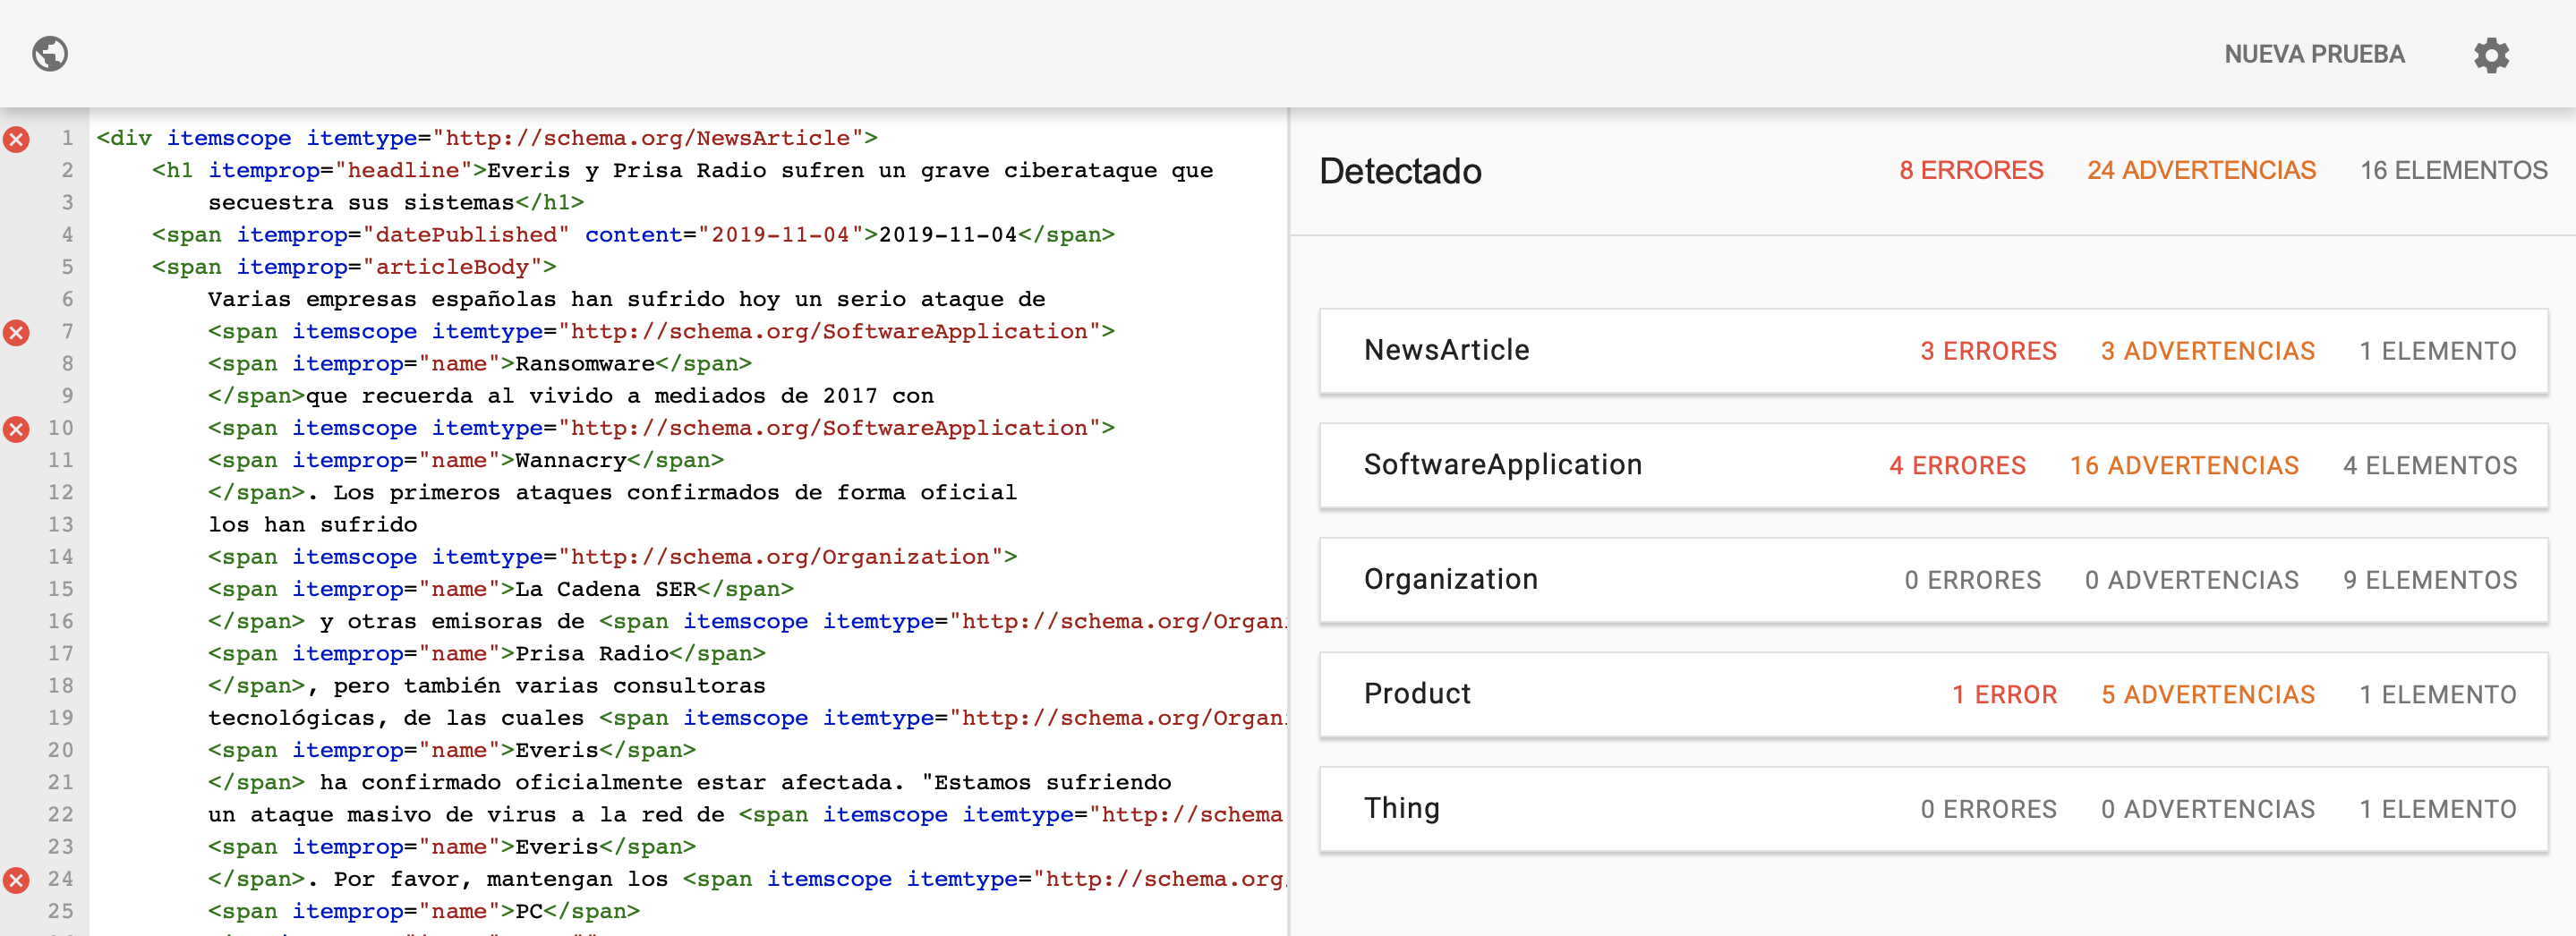
\includegraphics[width=\textwidth]{resources/testMicroData.png}
    \caption{Resultado del testeo del html con microdatos embebidos.}
    \label{Fig.1}
\end{figure}

Como se ve en la Fig.\ref{Fig.1} al validar el html generado este presenta errores y advertencias en las 
diferentes entidades, esto se debe a decisiones tomadas ante los incovenientes que presentan los microdatos, 
que se explicarán a continuación.

La entidad NewsArticle presenta los siguientes problemas:

\begin{itemize}
    \item Errores:
    \begin{itemize}
        \item Falta el atributo Author obligaotrio: Este es debido a que el extracto de la noticia no contiene esa información.
        \item Falta el atributo image obligaotrio: Este es debido a que el extracto de la noticia no contiene esa información.
        \item Falta el atributo publisher obligaotrio: Este es debido a que el extracto de la noticia no contiene esa información.
    \end{itemize}
    \item Advertencias:
    \begin{itemize}
        \item Falta el atributo DateModified recomendado: Este es debido a que el extracto de la noticia no contiene esa información.
        \item Falta el atributo mainEntityOfPage recomendado: Este es debido a que el extracto de la noticia no contiene esa información.
    \end{itemize}
\end{itemize}

Las 4 entidades SoftwareAplication presentan los mismos problemas:

\begin{itemize}
    \item Errores:
    \begin{itemize}
        \item En este caso el error es que son necesarios al menos dos de los atributos recomendados que se indican como advertencias a continuación.
    \end{itemize}
    \item Advertencias:
    \begin{itemize}
        \item Falta el atributo aggregateRating recomendado: Este es debido a que el extracto de la noticia no contiene esa información.
        \item Falta el atributo applicationCategory recomendado: Este es debido a que el extracto de la noticia no contiene esa información.
        \item Falta el atributo offers recomendado: Este es debido a que el extracto de la noticia no contiene esa información.
        \item Falta el atributo operatingSystem recomendado: Este es debido a que el extracto de la noticia no contiene esa información.
    \end{itemize}
\end{itemize}

La entidad Product presenta los siguientes problemas:

\begin{itemize}
    \item Errores:
    \begin{itemize}
        \item Falta el atributo offers obligaotrio: Este es debido a que el extracto de la noticia no contiene esa información.
        \item Falta el atributo review obligaotrio: Este es debido a que el extracto de la noticia no contiene esa información.
        \item Falta el atributo aggregateRating obligaotrio: Este es debido a que el extracto de la noticia no contiene esa información.
    \end{itemize}
    \item Advertencias:
    \begin{itemize}
        \item Falta el atributo brand recomendado: Este es debido a que el extracto de la noticia no contiene esa información.
        \item Falta el atributo description recomendado: Este es debido a que el extracto de la noticia no contiene esa información.
        \item Falta el atributo image recomendado: Este es debido a que el extracto de la noticia no contiene esa información.
        \item Falta el atributo sku recomendado: Este es debido a que el extracto de la noticia no contiene esa información.
        \item Falta algun atributo de tipo identificador global recomendado: Este es debido a que el extracto de la noticia no contiene esa información.
    \end{itemize}
\end{itemize}

\subsection{Cuestiones sobre el uso de microdatos.}

Ya realizado el proceso de los apartados anteriores queda plantearse las siguientes preguntas:

\textbf{\textit{¿Deberían tener valor para itemid todos los items? ¿Qué valor debería asignarse?}}

Depende, todos los itemid deberian tener un itemid de manera que se pudiera identificar cada uno de ellos unequivocamente, 
pero no en todos los casos, puesto que sobrecargaría los textos.
Además esto favorecería la propiedad de la web Semántica por la que toda entidad debe ser enlazable.

\textbf{\textit{¿Si hubiera varios candidatos cuál escogerías? ¿Por qué?}}.

En el caso de que hubiera varios candidatos para el identificador de un item elegiria un valor alfanumerico, como 
realiza WikiData por ejemplo, de este modo evitariamos colisiones y problemas de idiomas.

\textbf{\textit{¿Cuál crees que es la solución de compromiso que podría resultar menos polémica en la mayoría de casos?}}.

Para decidir si hay que añadir un itemid o no la solucion seria si ese item tiene un identificador, ya que quizas no lo tenga,
y si mejora la información que nos da.

\textbf{\textit{¿Qué inconvenientes concretos te ha supuesto la obligación de incrustarlos metadatos allí donde te "forzaba" 
la estructura del texto?}}.

El mayor problema que ha supesto incrustar los metadatos en la estructura del texto es que, por el modo 
en el que se hace cualquiera de ellos debe aparecer en el texto de manera que algunas propiedades obligatorias de las entidades
quedan sin rellenar porque no aparecen en el texto, y esto al revisarlo mediante la herramienta de Google da errores, 
que si quisieramos solucionar la unica manera posible para ello seria modificar el texto que se fuera a mostrar para que 
apareciesen todos los datos de la propiedades de cada entidad.

\section{JSON-LD}

A continuación se presentará la ultima version del jsonld que se facilita en la practica (Anexo.\ref{jsonld}), el cual se ha modificado 
de la siguiente forma:

\begin{itemize}
    \item Se han añadido a las entidades Periodical para que el id ahora sea la web oficial de la publicaciones.
    \item Se ha añadido al contexto del jsonld la url de DOI \textit{"https://doi.org/"}, y se han modificado las
        los items de tipo Chapter para que el id apunte a un \textit{"digital object identifier}.
    \item Se ha asociado al id de la entidad Person de Daniel Gayo su web oficial. Y de igual modo con las entidades 
    Universidad de Oviedo y Departamento de informatica con sus id's y las web's oficiales.
    \item Se han añadido a los items de tipo Periodical el atributo hasPart para señalar el articulo del que se habla de toda 
        la publicacion.
\end{itemize}

\lstset{
    frame=tb, % draw a frame at the top and bottom of the code block
    tabsize=2, % tab space width
    showstringspaces=false, % don't mark spaces in strings
    numbers=left, % display line numbers on the left
    commentstyle=\color{green}, % comment color
    keywordstyle=\color{red}, % keyword color
    stringstyle=\color{blue}, % string color    
    inputencoding=utf8/latin1
}
\lstinputlisting[language=HTML,breaklines,caption={Archivo HTML con JSONLD embebido.},captionpos=b]{resources/jsonld.html}

\section{Anexos}
\subsection{Extracto de la noticia seleccionada.}\label{noticia}
Varias empresas españolas han sufrido hoy un serio ataque de 'ransomware' que recuerda al 
vivido a mediados de 2017 con Wannacry. Los primeros ataques confirmados de forma oficial 
los han sufrido la Cadena SER y otras emisoras de Prisa Radio, pero también varias consultoras 
tecnológicas, de las cuales Everis ha confirmado oficialmente estar afectada. "Estamos sufriendo 
un ataque masivo de virus a la red de Everis. Por favor, mantengan los PCs apagados". Es el 
mensaje interno que ha remitido Everis a sus empleados, según ha podido confirmar este diario 
y han publicado también varios medios especializados. La compañía confirma que ha enviado a sus 
trabajadores a casa hasta que puedan solventar la incidencia.

"PRISA Radio ha sufrido esta madrugada un ataque de virus que ha tenido una afectación grave y 
generalizada de todos nuestros sistemas informáticos. Los técnicos especializados en este tipo 
de situaciones aconsejan encarecidamente la desconexión total de todos los sistemas con el fin 
de evitar la propagación del virus. Hablamos, por tanto, de una situación de extrema emergencia", 
ha comunicado esta mañana la empresa en un mensaje interno al que ha tenido acceso este diario.

"A partir de ese momento, se irá chequeando puesto a puesto -siguiendo las instrucciones precisas 
que os enviará el departamento de Sistemas- para autorizar en los casos en que haya garantía 
absoluta la puesta en marcha de cada equipo. Por el momento, y hasta nuevo aviso, la emisión de 
Cadena SER queda centralizada en Radio Madrid; quedan anuladas todas las emisiones locales y 
regionales, salvo aquellas que hayan sido autorizadas expresamente por la Dirección de Antena. 
En este momento, la seguridad es la máxima de la compañía por encima de cualquier otro compromiso. 
Cualquier acción individual no autorizada puede poner en peligro el trabajo de rescate que se está 
llevando a cabo", cierra el mensaje.

\subsection{JSONLD original}\label{jsonld}
\lstset{
    frame=tb, % draw a frame at the top and bottom of the code block
    tabsize=2, % tab space width
    showstringspaces=false, % don't mark spaces in strings
    numbers=left, % display line numbers on the left
    commentstyle=\color{green}, % comment color
    keywordstyle=\color{red}, % keyword color
    stringstyle=\color{blue}, % string color    
    inputencoding=utf8/latin1
}
\lstinputlisting[breaklines,caption={JSON Original facilitado en la practica.},captionpos=b]{resources/jsonOriginal.json}

\end{document}